\documentclass[a4paper, 11pt]{article}

\usepackage{parskip}
\usepackage{hyperref}
\hypersetup{ colorlinks, citecolor=green, filecolor=black, linkcolor=blue, urlcolor=blue } 

\usepackage{colortbl}

\usepackage{amsfonts}

\usepackage[left=2cm, right=2cm, top=2cm]{geometry}
\usepackage{float}
\usepackage{afterpage}
\usepackage{multirow}
\usepackage{listings}
\usepackage{xcolor}
 
\definecolor{codegreen}{rgb}{0,0.6,0}
\definecolor{codegray}{rgb}{0.5,0.5,0.5}
\definecolor{codepurple}{rgb}{0.58,0,0.82}
\definecolor{backcolour}{rgb}{0.95,0.95,0.92}
 
\lstdefinestyle{mystyle}{
    backgroundcolor=\color{backcolour},   
    commentstyle=\color{codegreen},
    keywordstyle=\color{magenta},
    numberstyle=\tiny\color{codegray},
    stringstyle=\color{codepurple},
    basicstyle=\ttfamily\footnotesize,
    breakatwhitespace=false,         
    breaklines=true,                 
    captionpos=b,                    
    keepspaces=true,                 
    numbers=left,                    
    numbersep=5pt,                  
    showspaces=false,                
    showstringspaces=false,
    showtabs=false,                  
    tabsize=2
}
\lstset{style=mystyle}

\usepackage{gensymb}
\usepackage{amsmath}
\usepackage{graphicx}
\usepackage{subfigure}
\usepackage{textcomp}
\usepackage{enumitem}

\newcommand{\points}[1]{(\textbf{#1 marks}) }
\newcommand{\vecthree}[3]{\begin{pmatrix} #1 \\ #2 \\ #3 \end{pmatrix}}
\newcommand{\vecfour}[4]{\begin{pmatrix} #1 \\ #2 \\ #3 \\ #4\end{pmatrix}}
\newcommand{\mat}[1]{\boldsymbol { \mathsf{#1}} }

\DeclareMathOperator*{\argmax}{arg\,max}
\DeclareMathOperator*{\argmin}{arg\,min}
\newcommand{\norm}[1]{\lVert#1\rVert}
\newcommand{\R}{\mathbb{R}}

\definecolor{mycolor}{rgb}{0,0.6,0.5}

\title{CS340/MATH321 -- Geometrical modelling and numerical analysis \\ Group project 2}
\vspace{-10em}
\date{Fall 2019}
\author{Huda Feroz Ahmed \and Aiman Khan \and Muhammad Shahrom Ali}

\begin{document}
\maketitle  
\setlength{\parskip}{10pt}
\setlength{\parindent}{0pt}
\DeclareGraphicsExtensions{.pdf,.png,.gif,.jpg}

\begin{enumerate}
    
\item \textbf{(50 points)} The following question asks you to explore and implement the equation \[\vec p(s, t) = \sum N_i(s, t) \vec p_i\] in two- and three-dimensions

\begin{enumerate}[label=\alph*.]
    \item \textbf{(3 points)} Draw all the linear and quadratic B\'{e}zier basis functions over a unit interval and a unit square
    \subsection*{Solution}
    Figure \ref{fig:bezierBasisCurve} represents the linear and quadratic B\'{e}zier basis functions over a unit interval. The following code has been used to generate the figures \ref{fig:bezierBasisCurve} and \ref{fig:bezierBasisSurface}. Use \texttt{type="curve"} to generate basis functions over a unit interval, and use \texttt{type="surface"} to generate basis functions over a unit square.
    \begin{lstlisting}[language=Python]
plotBezierBasisFunctions(type='curve',degree=1)
plotBezierBasisFunctions(type='curve',degree=2)
plotBezierBasisFunctions(type='surface',degree=1)
plotBezierBasisFunctions(type='surface',degree=2)
\end{lstlisting} 
    \begin{figure}[ht] 
  \subfigure[Linear Bezier basis]{% 
    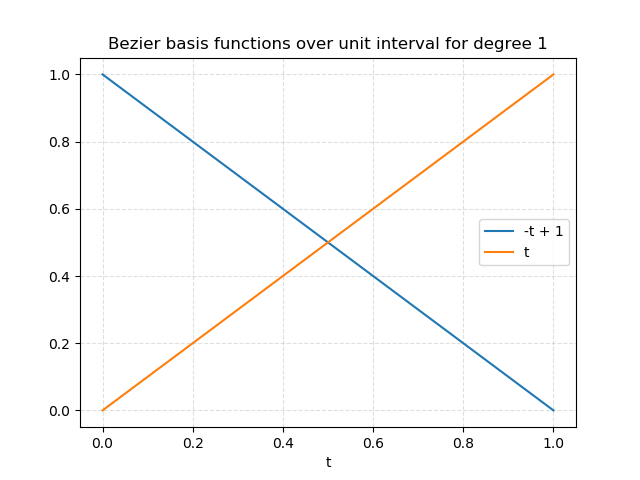
\includegraphics[scale=0.5]{resources/bezierBasisFunctionCurve1.png} \label{fig:bezierBasisCurve1} 
  } 
 \quad 
  \subfigure[Quadratic Bezier basis]{% 
    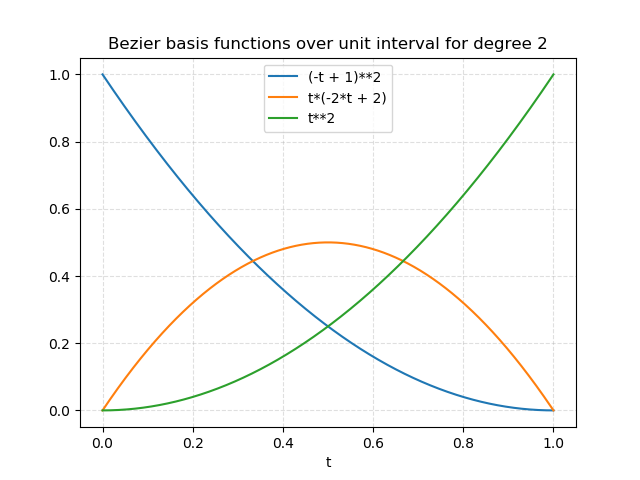
\includegraphics[scale=0.5]{resources/bezierBasisFunctionCurve2.png} \label{fig:bezierBasisCurve2} 
  } 
  \caption{Bezier Basis over Unit Interval} 
  \centering
  \label{fig:bezierBasisCurve}
\end{figure} 
\clearpage
Figure \ref{fig:bezierBasisSurface} represents the linear and quadratic B\'{e}zier basis functions over a unit square: 
\begin{figure}[ht] 
  \subfigure[Linear Bezier basis]{% 
    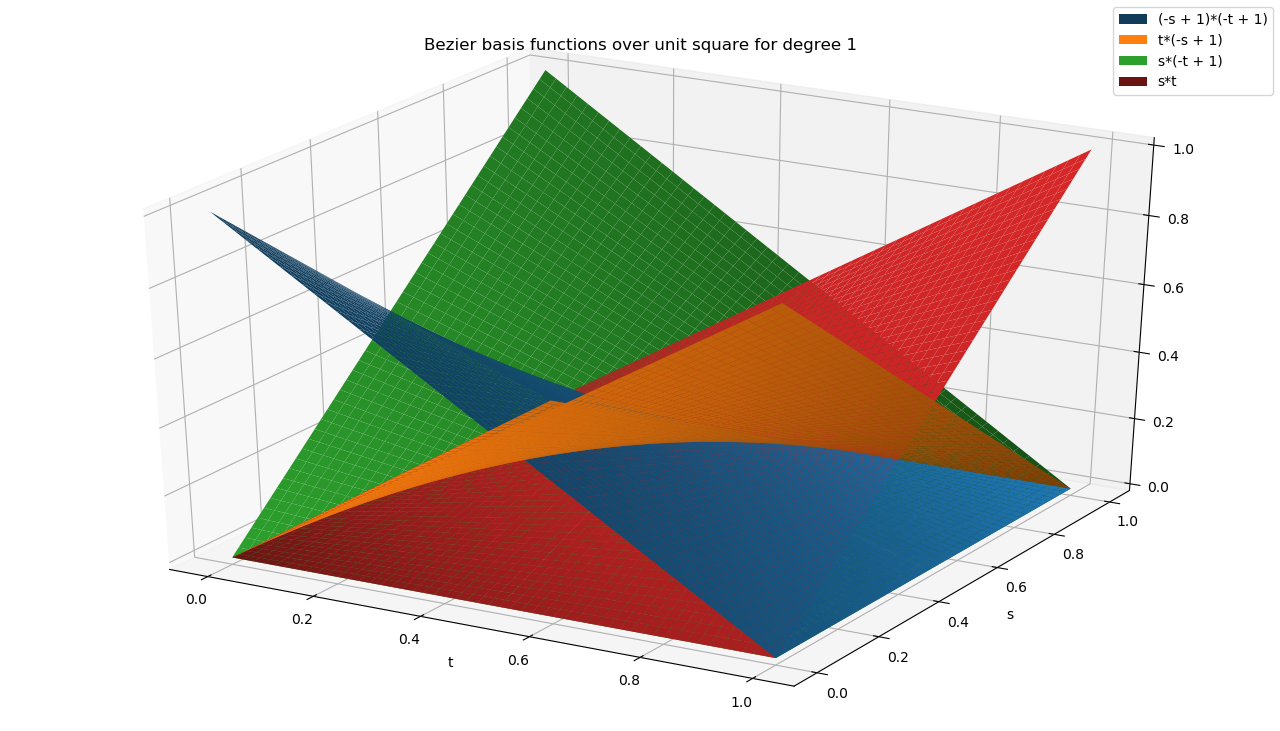
\includegraphics[scale=0.25]{resources/bezierBasisFunctionSurface1.png} \label{fig:bezierBasisSurface1} 
  } 
 \quad 
  \subfigure[Quadratic Bezier basis]{% 
    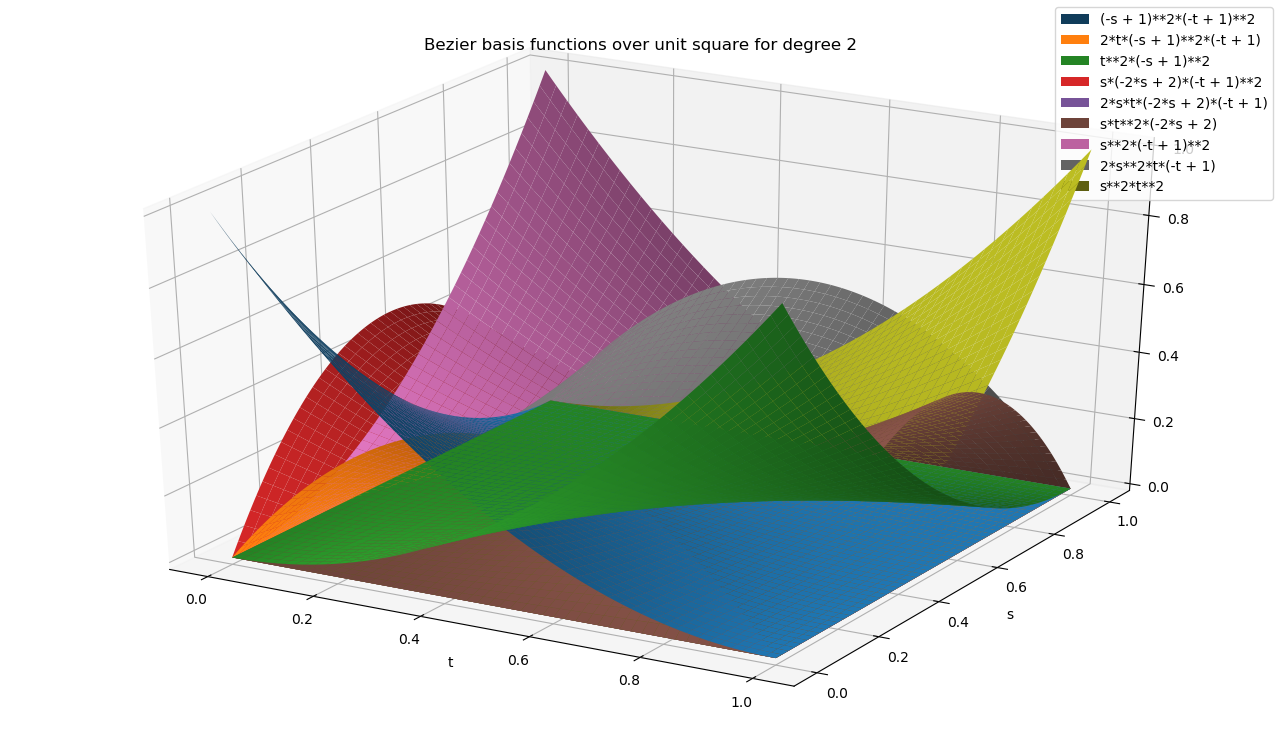
\includegraphics[scale=0.25]{resources/bezierBasisFunctionSurface2.png} \label{fig:bezierBasisSurface2} 
  } 
  \caption{Bezier Basis over Unit Square} 
  \label{fig:bezierBasisSurface}
\end{figure}
    \item \textbf{(3 points)} Draw a linear, quadratic, cubic, quartic b-splines basis functions in 1D over a uniform knot vector 
    \subsection*{Solution}
    Figure \ref{fig:bsplineBasis} represents the b-spline basis functions for uniform knot vector \([0,1,2,3,4,5,6]\) and the following code has been used to generate it. 
    \begin{lstlisting}[language=Python]
knot_vector = [0,1,2,3,4,5,6]
plotBsplineBasisFunctions(knot_vector,2) #linear
plotBsplineBasisFunctions(knot_vector,3) #Quadratic
plotBsplineBasisFunctions(knot_vector,4) #Cubic
plotBsplineBasisFunctions(knot_vector,5) #Quartic
\end{lstlisting} 
    \begin{figure}[ht] 
  \subfigure[Linear b-spline basis]{% 
    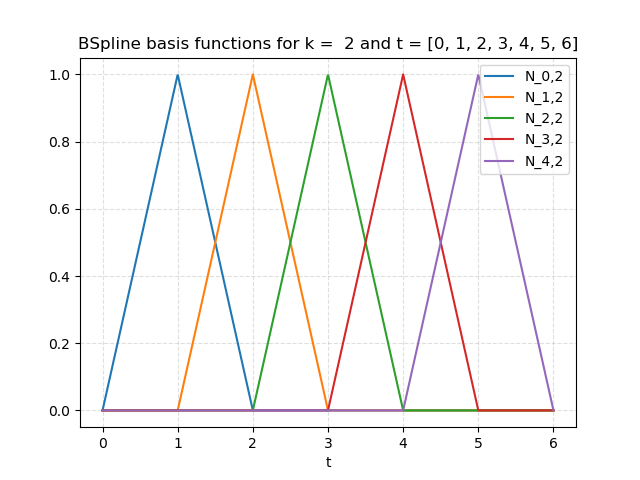
\includegraphics[scale=0.5]{resources/bSplineBasisk2.png} \label{fig:linearBSpline}
  } 
 \quad 
  \subfigure[Quadratic b-spline basis]{% 
    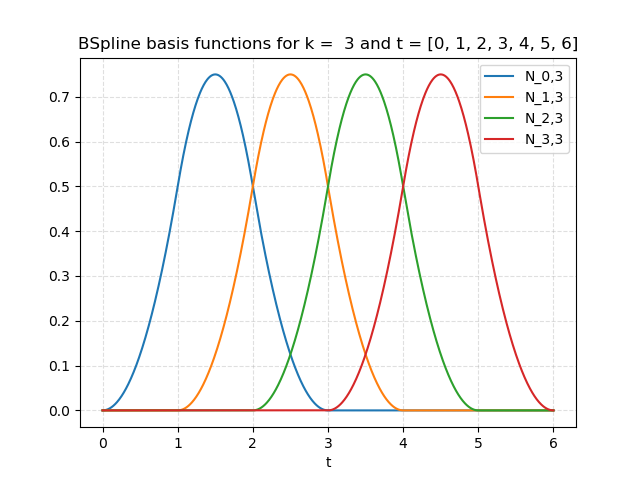
\includegraphics[scale=0.5]{resources/bSplineBasisk3.png} \label{fig:quadraticBSpline} 
  } \\
  \quad 
  \subfigure[Cubic b-spline basis]{% 
    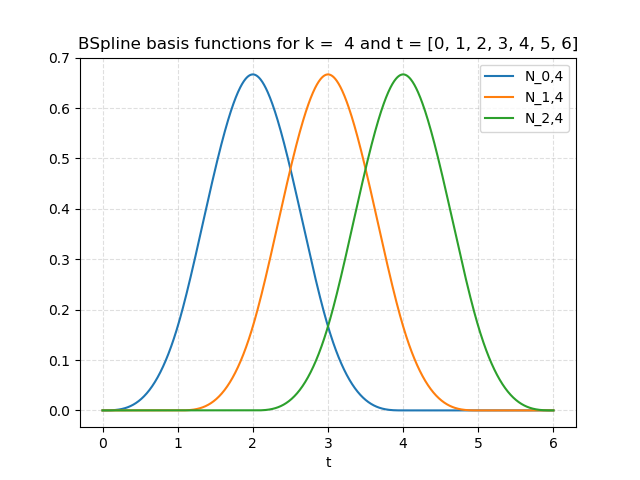
\includegraphics[scale=0.5]{resources/bSplineBasisk4.png} \label{fig:cubicBSpline} 
  }
  \quad 
  \subfigure[Quartic b-spline basis]{% 
    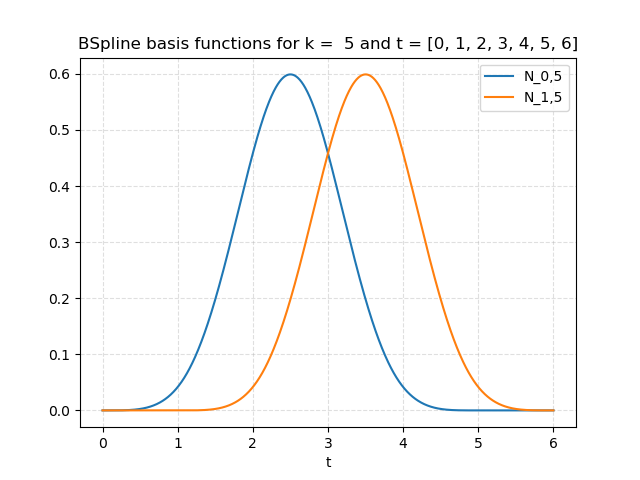
\includegraphics[scale=0.5]{resources/bSplineBasisk5.png} \label{fig:quarticBSpline} 
  }
  \caption{B-Spline Basis for knot vector \([0,1,2,3,4,5,6]\)} 
  \label{fig:bsplineBasis}
\end{figure}
    \item \textbf{(3 points)} Draw quadratic, cubic, and quartic B\'{e}zier curves by arbitrary defining the appropriate control points 
    \subsection*{Solution}
    Figure \ref{fig:bezierCurves} represents the different bezier curves formed and has been generated through the following code.
    \begin{lstlisting}[language=Python]
curveCP = {1:[[0,0],[0.5,1]], 
           2: [[1,2],[0,0],[2,0]],
           3:[[0,0],[0.5,1],[0.5,0],[1,1]],
           4:[[0,0],[1,0],[1,1],[0,1],[0.5,2]]}  
           
plotBezierCurves(curveCP[2],2) #Quadratic
plotBezierCurves(curveCP[3],3) #Cubic
plotBezierCurves(curveCP[4],4) #Quartic
\end{lstlisting} 
        \begin{figure}[ht] 
  \subfigure[Quadratic Bezier Curve]{% 
    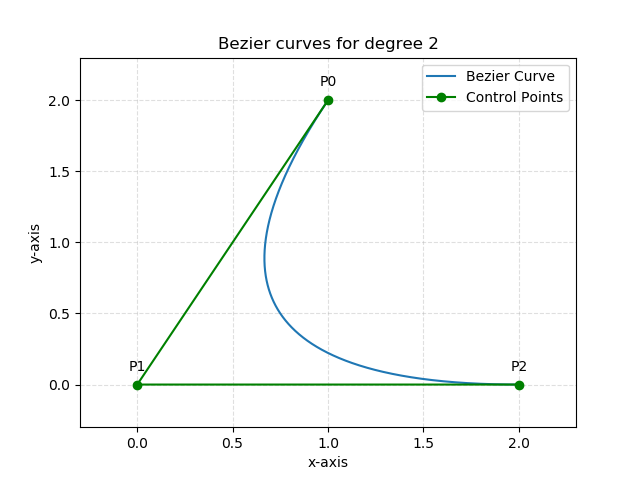
\includegraphics[scale=0.5]{resources/QuadraticBezierCurve.png} \label{fig:quadraticBezierCurve} 
  } 
 \quad 
  \subfigure[Cubic Bezier Curve]{% 
    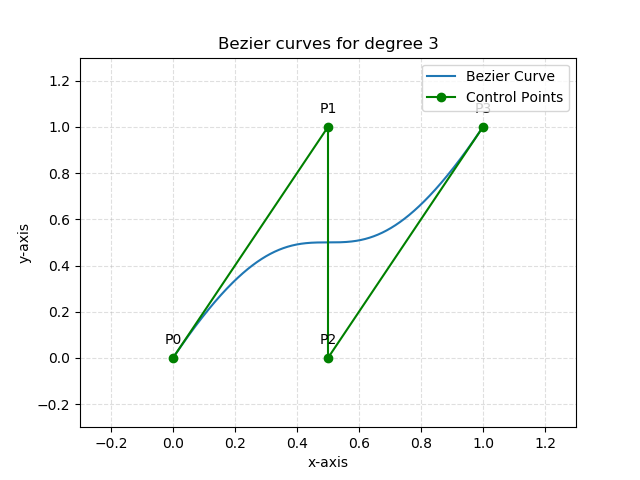
\includegraphics[scale=0.5]{resources/CubicBezierCurve.png} \label{fig:cubicBezierCurve} 
  } \\
  \quad 
  \subfigure[Quartic Bezier Curve]{% 
    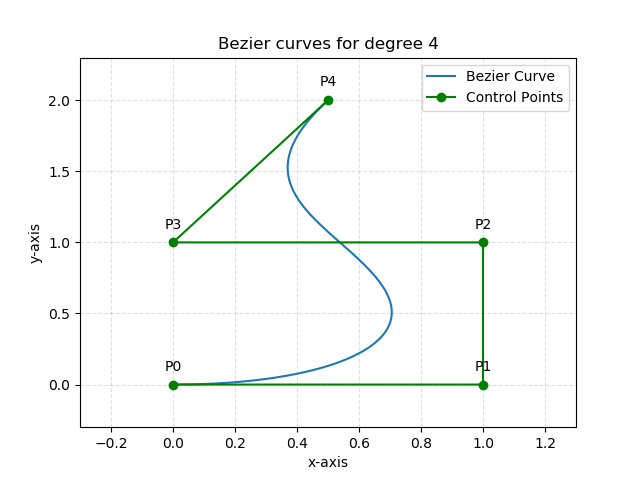
\includegraphics[scale=0.5]{resources/QuarticBezierCurve.png} \label{fig:quaricBezierCurve} 
  }
  \caption{Bezier Curves of different degrees} 
  \label{fig:bezierCurves}
\end{figure}
\clearpage
    \item \textbf{(6 points)} The curve generated using B\'{e}zier basis functions do not usually pass through the control points. Derive new quadratic and cubic polynomial basis functions $N_i(t)$ which when linearly combined with the control points $\vec p_i$ will generate a curve which passes through the control points. Draw them and comment on potential advantages and disadvantages of these basis functions. You can define the control points arbitrarily. 
    \subsection*{Solution}
    The curve generated using B\'{e}zier basis functions only passes through the first and last control points because the first and last basis function is equal to 1 at some value of parametric coordinate $t$.
    For quadratic bezier curves \((1-t)^2 = 1\) at \(t=0\) and \(t^2=1\) at \(t=1\). Similarly, for cubic bezier curves \((1-t)^3 = 1\) at \(t=0\) and \(t^3=1\) at \(t=1\). Other basis functions, for quadratic and cubic both do not equal to 1 at any value of \( t \in [0,1] \). In order to make bezier curve pass through control points, we need to derive new basis which equal to 1 at some \(t\).
    \subsubsection*{New Quadratic Basis}
    For quadratic basis, lets say we want the basis function equal to 1 at \(t=0\), \(t=0.5\) and \(t=1\). We can have three terms \(t\), \((1-t)\) and \((0.5-t)\). \\
    We want the first basis function to be equal to 1 at \(t=0\), for this we have to choose \((1-t)(0.5-t)\). Similarly, we want the second basis function to be equal to 1 at \(t=0.5\), for this we have to choose \((1-t)(t)\). And similarly, we want the third basis function to be equal 1 at \(t=1\), for this we have to choose \((0.5-t)t\). Hence the new basis functions are:
    \begin{equation}
        \label{quadraticNewBasis}
        (1-t)(0.5-t) ; (1-t)(t) ; (0.5-t)t
    \end{equation}
    These basis functions are all quadratic in nature just like original basis functions for quadratic curves but they do not equal to 1 at desired \(t\) values. To make them equal to 1 we need to multiply them with some constants. Hence the new basis functions for quadratic bezier curves which pass through control points are given as:
    \begin{equation}
        \label{quadraticNewBasis1}
        2(1-t)(0.5-t) ;\hspace{0.5cm} 4(1-t)(t) ; \hspace{0.5cm} -2(0.5-t)t
    \end{equation}
    \subsubsection*{New Cubic Basis}
    For cubic basis, we will do the exact same steps as we did for quadratic, but since now there are 4 terms, we want the basis function to be equal to 1 at \(t=0\), \(t=\frac{1}{3}\), \(t = \frac{2}{3}\) and \(t=1\). We can have 4 terms \(t\), \((1-t)\), \((\dfrac{1}{3}-t)\) and \((\frac{2}{3}-t)\). \\
    We want the first basis function to be equal to 1 at \(t=0\), for this we have to choose \((1-t)(\frac{1}{3}-t)(\frac{2}{3}-t)\). Similarly, we want the second basis function to be equal to 1 at \(t=\frac{1}{3}\), for this we have to choose \((1-t)(t)(\frac{2}{3}-t)\). For third basis function to be equal 1 at \(t=\frac{2}{3}\), we have to choose \((\frac{1}{3}-t)(t)(1-t)\). Finally, for last the basis function to be equal to 1 at \(t = 1\), we have to choose \((t)(\frac{1}{3}-t)(\frac{2}{3}-t)\). These functions still do not equal to 1 at specified \(t\) values, hence we will add some constants. Hence the new basis functions are:
    \begin{equation}
        \label{cubicNewBasis}
        \frac{9}{2}(1-t)(\frac{1}{3}-t)(\frac{2}{3}-t) ; \hspace{0.5cm} \frac{27}{2}(1-t)(t)(\frac{2}{3}-t) ;
        \hspace{0.5cm}
        \frac{-27}{2}(1-t)(t)((\frac{1}{3}-t);
        \hspace{0.5cm}
        \frac{9}{2}(t)(\frac{1}{3}-t)(\frac{2}{3}-t)
    \end{equation}
    \subsubsection*{Advantages}
    An advantage of such a basis is that we can still reach a certain control point by substituting different values of \(t\). For example, for new quadratic basis, at \(t = 0\), we are at point \(P_0\). Similarly at \(t=0.5\), we are at point \(P_1\). And same goes for cubic basis. 
    \subsubsection*{Disadvantages}
    A major disadvantage of these new basis functions is that that they are not an affine combination anymore. As we can see in the graphs that the curved spanned by these control points now goes outside the control polygon.  \\ \\
    Figure \ref{fig:bezierCurvesCP} represents the bezier curves passing through control points. and has been generated using the following code. 
    \begin{lstlisting}[language=Python]
curveCP = {1:[[0,0],[0.5,1]], 
           2: [[1,2],[0,0],[2,0]],
           3:[[0,0],[0.5,1],[0.5,0],[1,1]],
           4:[[0,0],[1,0],[1,1],[0,1],[0.5,2]]}  
           
newBezierBasisToPassThroughCP(curveCP[2],2) #Quadratic
newBezierBasisToPassThroughCP(curveCP[3],3) #Cubic
\end{lstlisting} 
    \begin{figure}[ht] 
  \subfigure[Quadratic Bezier Curve]{% 
    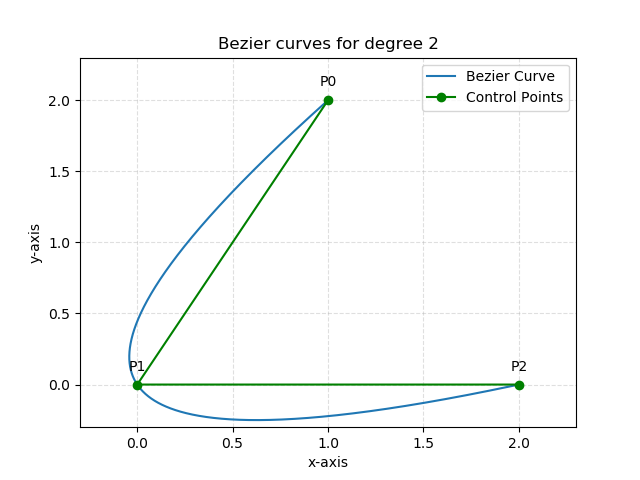
\includegraphics[scale=0.5]{resources/quadraticCurveCP.png} \label{fig:quadraticBezierCurveCP} 
  } 
 \quad 
  \subfigure[Cubic Bezier Curve]{% 
    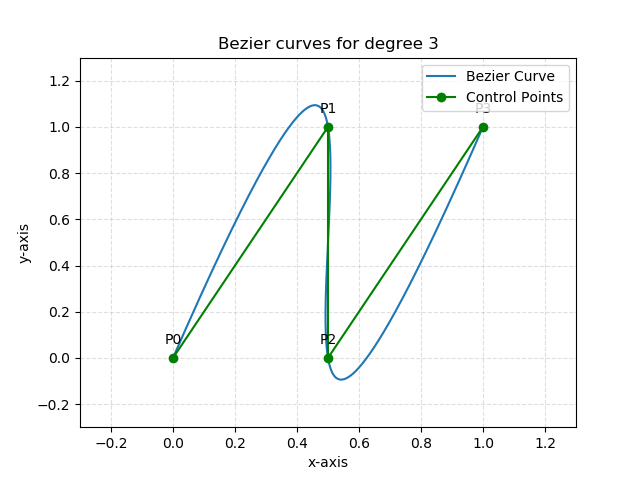
\includegraphics[scale=0.5]{resources/cubicCurveCP.png} \label{fig:cubicBezierCurveCP} 
  }
  \caption{Bezier Curves passing through control points.} 
  \label{fig:bezierCurvesCP}
\end{figure}
    \item \textbf{(6 points)} Now imagine you have a cubic B\'{e}zier curves $\vec P(t)$ and $\vec Q(t)$, derive the conditions on the control points such that the curves $\vec P(t)$ join the curve $\vec Q(t)$ with $C^1$ and with $C^2$ continuity. What is the continuity of the cubic B\'{e}zier curve $\vec P(t)$ by itself.
    \subsection*{Solution}
    The equations for cubic bezier curves \(P(t)\) and \(Q(t)\) can be written as:
    \begin{equation}
    \label{eq:p(t)}
        P(t) = (t-1)^3 P_0 + 3(t-1)^2 t P_1 + 3(t-1) t^2 P_2 + t^3 P_3 
    \end{equation}
    \begin{equation}
    \label{eq:q(t)}
        Q(t) = (t-1)^3 Q_0 + 3(t-1)^2 t Q_1 + 3(t-1) t^2 Q_2 + t^3 Q_3 
    \end{equation}
    To ensure, \(C^0\) continuity, equation \ref{eq:c0} should satisfy
    \begin{equation}
        \label{eq:c0}
        P(1) = Q(0)
    \end{equation}
    Following from equation \ref{eq:c0} we have:
    \begin{equation}
        \label{eq:c0-1}
        P_3 = Q_0
    \end{equation}
    To ensure, \(C^1\) continuity, equation \ref{eq:c1} should satisfy
    \begin{equation}
        \label{eq:c1}
        P'(1) = Q'(0)
    \end{equation}
    Following from equation \ref{eq:c1} we have:
    \begin{equation}
        \label{eq:c1-1}
        -3P_2 + 3P_3 = -3Q_0 + 3Q_1
    \end{equation} 
    By simplifying equation \ref{eq:c1-1} and substituting the value of \(Q_0\) from equation \ref{eq:c0-1} we get the conditions on the control points such that the curve \(\vec P(t) \) joins the curve \(\vec Q(t)\) with \(C^1\) continuity:
    \begin{equation}
        \label{eq:c1-2}
        \boxed{2P_3 - P_2 = Q_1}
    \end{equation}
    To ensure, \(C^2\) continuity, equation \ref{eq:c2} should satisfy
    \begin{equation}
        \label{eq:c2}
        P''(1) = Q''(0)
    \end{equation}
    Following from equation \ref{eq:c2} we have:
    \begin{equation}
        \label{eq:c2-1}
       6P_1 - 12P_2 + 6P_3 = 6Q_0 - 12Q_1 + 6Q_2
    \end{equation} 
    By simplifying equation \ref{eq:c2-1} and substituting the value of \(Q_0\) from equation \ref{eq:c0-1} we get the conditions on the control points such that the curve \(\vec P(t) \) joins the curve \(\vec Q(t)\) with \(C^2\) continuity:
    \begin{equation}
        \label{eq:c2-2}
        P_1 - 2P_2 = -2Q_1 + Q_2
    \end{equation}
    Using the constraints for \(C^1\) continuity, we can substitute the value of \(Q_1\) from equation \ref{eq:c1-2}, to obtain the simplified condition for \(C^2\) continuity:
    \begin{equation}
        \label{eq:c2-final}
        \boxed{P_1 - 4P_2 + 4P_3 = Q_2}
    \end{equation}
    The continuity of the cubic B\'{e}zier curve $\vec P(t)$ by itself is \(C^n\) $\forall n$ because any bezier curve is infinitely differentiable within itself, and is therefore continuous to any degree (\(C^n\)-continuous, $\forall n$) \cite{bezier}. 
    \item \textbf{(9 points)} For part e), draw a figure which demonstrates that the curve $\vec P(t)$ joins the curve $\vec Q(t)$ with $C^1$ continuity. Draw a similar figure(s) which demonstrates that the curves join with $C^2$ continuity. The figure must be generated by some algorithm/function. 
    \subsection*{Solution}
    Using the conditions obtained in part e, we can draw the curves which join with desired continuity. Figure \ref{fig:bezierCurvesJoined} represents the curves \(P(t)\) and \(Q(t)\) joined by different continuities and has been generated using the following code.
    \begin{lstlisting}[language=Python]
cpP = [[0,0],[0.5,1],[0.5,0],[1,1] #control points for P
cpQ = [[1.5,1.5],[2,2.5],[2,1.5],[2.5,2.5]] #control points for Q
cubicBezierCurvesJoinedWithContinuity(continuity='C-1',cpP=cpP,cpQ=cpQ) 
cubicBezierCurvesJoinedWithContinuity(continuity='C0',cpP=cpP,cpQ=cpQ)
cubicBezierCurvesJoinedWithContinuity(continuity='C1',cpP=cpP,cpQ=cpQ)
cubicBezierCurvesJoinedWithContinuity(continuity='C2',cpP=cpP,cpQ=cpQ)
\end{lstlisting} 
    \begin{figure}[ht] 
  \subfigure[Curves joined by \(C^{-1}\) continuity]{% 
    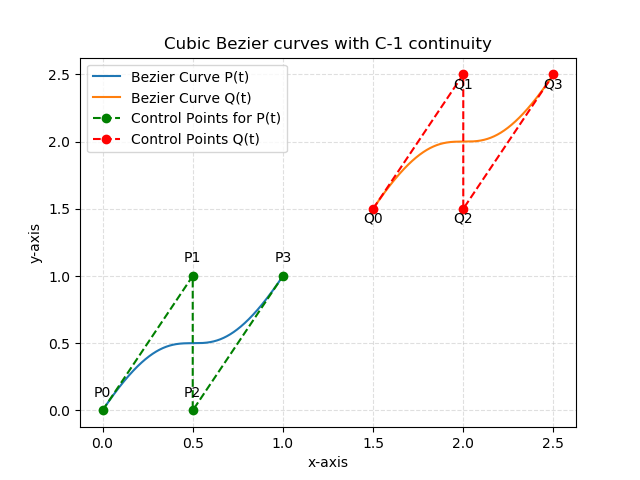
\includegraphics[scale=0.5]{resources/BezierC-1.png} \label{fig:c-1} 
  } 
 \quad 
  \subfigure[Curves joined by \(C^{0}\) continuity]{% 
    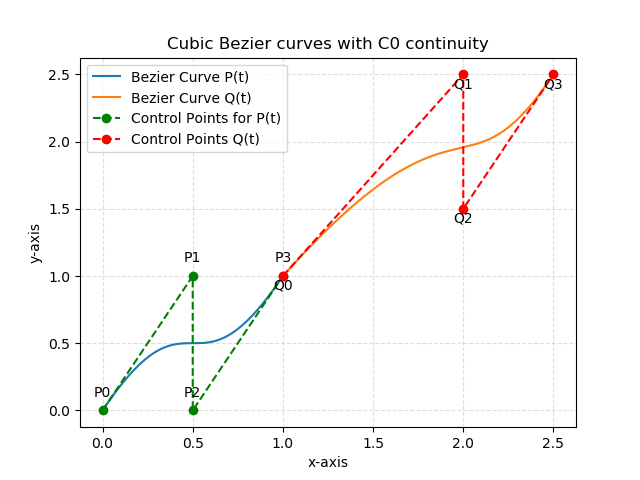
\includegraphics[scale=0.5]{resources/BezierC0.png} \label{fig:c0} 
  } \\
  \quad 
  \subfigure[Curves joined by \(C^{1}\) continuity]{% 
    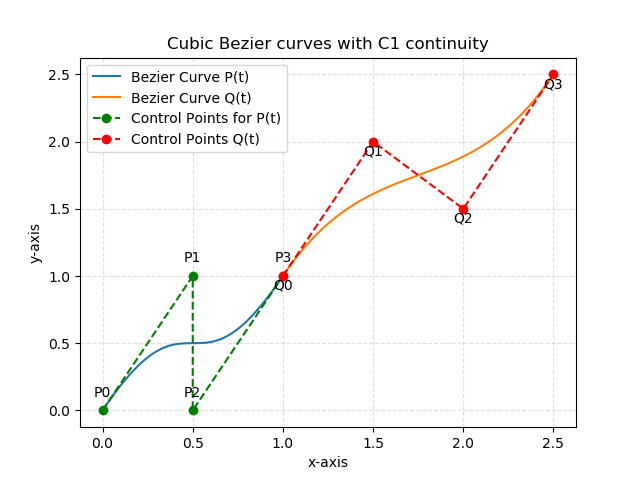
\includegraphics[scale=0.5]{resources/BezierC1.png} \label{fig:c1} 
  }
  \quad 
  \subfigure[Curves joined by \(C^{2}\) continuity]{% 
    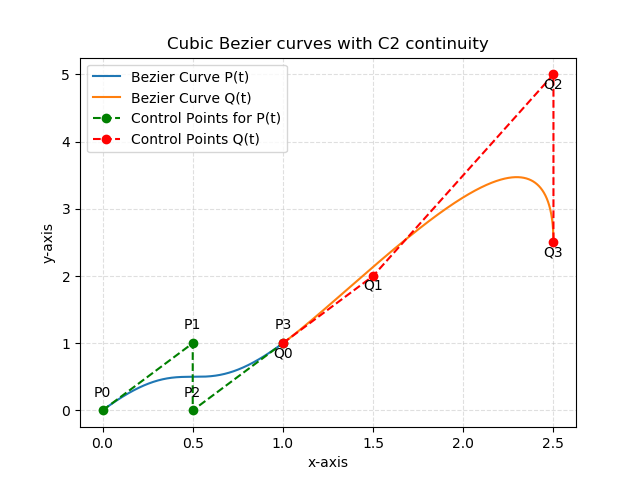
\includegraphics[scale=0.5]{resources/BezierC2.png} \label{fig:c2} 
  }
  \caption{Cubic Bezier Curves \(P(t)\) and \(Q(t)\) joined by different continuities.} 
  \label{fig:bezierCurvesJoined}
\end{figure}
\clearpage
    \item \textbf{(9 points)} Repeat parts c-d for a single patch with tensor product structure
    \subsection*{Solution}
    Figures \ref{fig:QuadraticPatch}, \ref{fig:CubicPatch},\ref{fig:QuarticPatch} represents the different bezier patches formed and has been generated through the following code. 
    \begin{lstlisting}[language=Python]
patchCP = {2 : [[0,0,10],[3,0,-10],[6,0,0],[0,3,12],
                [3,3,0],[6,3,0],[0,6,0],[3,6,4],[6,6,0]],
           3 : [[0,0,0], [1,0,2], [2,0,-1],[3,0,0],
               [0,1,0], [1,1,4], [2,1,4], [3,1,0],
               [0,2,0], [1,2,8], [2,2,8],  [3,2,0],
               [0,3,0], [1,3,0], [2,3,0], [3,3,0]],
           4 : [[0,0,0], [1,0,2], [2,0,-1],[3,0,0],
               [0,1,0], [1,1,4], [2,1,4], [3,1,4], [3,2,4], [3,1,0],
               [0,2,0], [1,2,8], [2,2,8], [2,4,8], [4,2,8],  [3,2,0],
               [0,3,0], [1,3,0], [2,3,0], [3,3,0], [3,2,1],
               [0,3,1], [1,3,1], [2,3,1], [3,3,1]
           ]}
plotBezierSurfaces(patchCP[2],2) #Quadratic
newBezierSurfacesThroughCP(patchCP[2],2) #Quadratic Through CP
plotBezierSurfaces(patchCP[3],3) #Cubic
newBezierSurfacesThroughCP(patchCP[3],3) #Cubic Through CP
plotBezierSurfaces(patchCP[4],4) #Quartic
\end{lstlisting}  
The new basis for quadratic and cubic bezier patches are given in code file, and has been derived by just replacing the following in the original basis for both $s$ and $t$. For Quadratic, replace:
\begin{align*}
    (1-t)^2 \longrightarrow   2(1-t)(0.5-t) \\ 
    2t(1-t) \longrightarrow 4(1-t)(t) \\
    t^2 \longrightarrow -2(0.5-t)t 
\end{align*}
For cubic, replace (for both $s$ and $t$):
\begin{align*}
    (1-t)^3 \longrightarrow   \frac{9}{2}(1-t)(\frac{1}{3}-t)(\frac{2}{3}-t) \\ 
    3t(1-t)^2 \longrightarrow \frac{27}{2}(1-t)(t)(\frac{2}{3}-t)\\
    3t^2(1-t) \longrightarrow \frac{-27}{2}(1-t)(t)((\frac{1}{3}-t) \\
    t^3 \longrightarrow \frac{9}{2}(t)(\frac{1}{3}-t)(\frac{2}{3}-t)
\end{align*}
\clearpage
     \begin{figure}[ht] 
  \subfigure[Quadratic Bezier Patch]{% 
    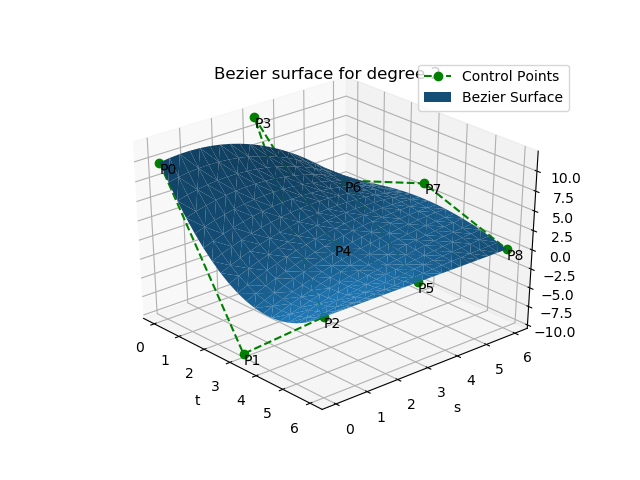
\includegraphics[scale=0.6]{resources/bezierSurface2.png} \label{fig:quadraticBezierPatch} 
  } 
 \quad 
  \subfigure[Quadratic Bezier patch passing through control points]{% 
    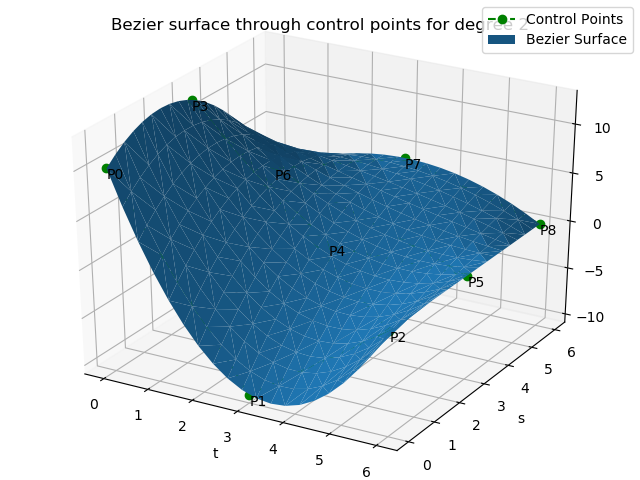
\includegraphics[scale=0.5]{resources/bezierSurfaceCP2.png} \label{fig:quadraticBezierPatchCP} 
  }
  \caption{Quadratic Bezier Patches} 
  \label{fig:QuadraticPatch}
\end{figure}
\begin{figure}[ht] 
  \subfigure[Cubic Bezier Patch]{% 
    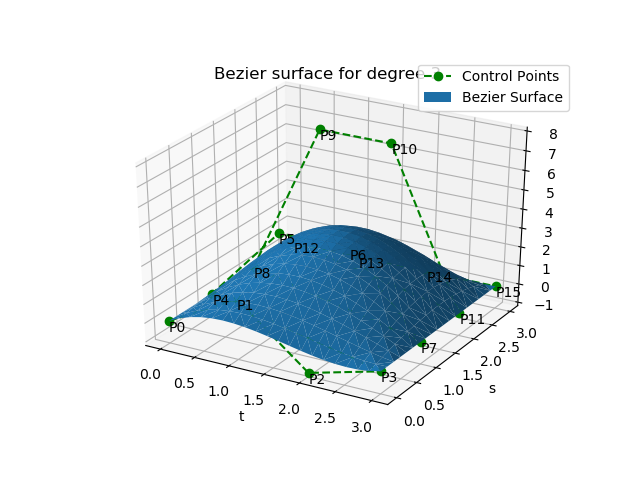
\includegraphics[scale=0.6]{resources/bezierSurface3.png} \label{fig:cubicBezierPatch} 
  } 
 \quad 
  \subfigure[Cubic Bezier patch passing through control points]{% 
    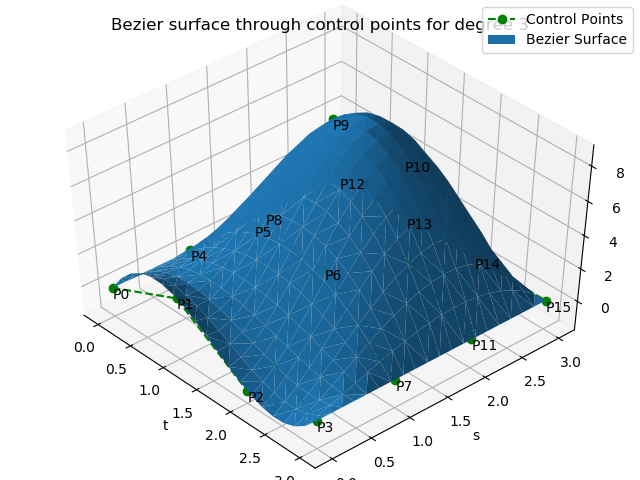
\includegraphics[scale=0.5]{resources/bezierSurfaceCP3.png} \label{fig:cubicBezierPatchCP} 
  }
  \caption{Cubic Bezier Patches} 
  \label{fig:CubicPatch}
\end{figure}
\clearpage
\begin{figure}[ht] 
  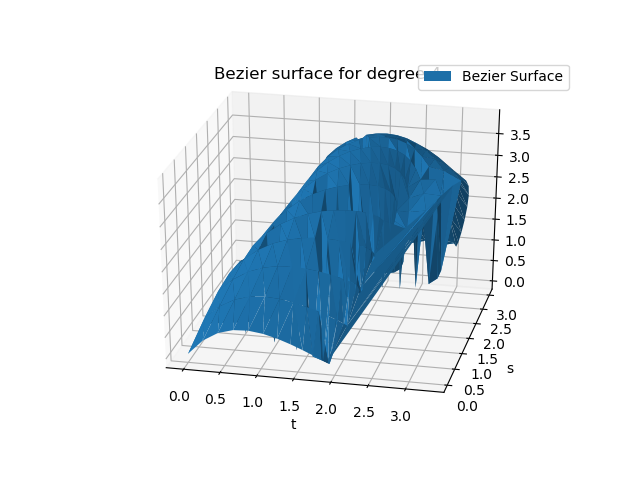
\includegraphics[scale=0.7]{resources/bezierSurface4.png}
  \centering
  \caption{Quartic Bezier Path} 
  \label{fig:QuarticPatch}
\end{figure}
    \item \textbf{(2 points)} Consider two arbitrary tensor product quadratic B\'{e}zier patches $\vec P(s,t)$ and $\vec Q(s,t)$, describe (qualitatively or mathematically) the conditions for $C^1$ continuity along the edge at which they meet?
    \subsection*{Solution}
    \underline{Assumption}: Let we are limiting our problem such that the patches meet at one boundary. \\ \\
    We have taken the points in the following order, assuming $t$ on the vertical axis, and $s$ on the horizontal axis. 
    \begin{align*}
        P_{2,0} , P_{2,1},  P_{2,2} \\ 
        P_{1,0} , P_{1,1},  P_{1,2} \\ 
        P_{0,0} , P_{0,1},  P_{0,2} \\
    \end{align*}
    The same alignment is assumed for control points of patch \(Q(s,t)\). \\ \\
    The equations for quadratic bezier patches \(P(s,t)\) and \(Q(s,t)\) can be written as:
    \begin{multline}
    \label{eq:p(s,t)}
        P(s,t) = (1-s)^2[(1-t)^2 P_{0,0} + 2t(1-t) P_{0,1} + t^2 P_{0,2}] + \\ 2s(1-s)[(1-t)^2 P_{1,0} + 2t(1-t) P_{1,1} + t^2 P_{1,2}] + \\
        s^2[(1-t)^2 P_{2,0} + 2t(1-t) P_{2,1} + t^2 P_{2,2}]
    \end{multline}
    \begin{multline}
    \label{eq:q(s,t)}
        Q(s,t) = (1-s)^2[(1-t)^2 Q_{0,0} + 2t(1-t) Q_{0,1} + t^2 Q_{0,2}] + \\ 2s(1-s)[(1-t)^2 Q_{1,0} + 2t(1-t) Q_{1,1} + t^2 Q_{1,2}] + \\
        s^2[(1-t)^2 Q_{2,0} + 2t(1-t) Q_{2,1} + t^2 Q_{2,2}]
    \end{multline}
    To ensure \(C^0\) continuity,  both the curves should meet at boundary, they should share control points at the edge. Boundary of a bezier patch is obtained when either of the parametric coordinate equals to 1 or 0, while the other coordinate ranges from 0 to 1. Since we are dealing with just one boundary, we can fix either of the parametric coordinates to a specific value (lets say $t=1$ for $P(s,t)$ and $t=0$ for $Q(s,t)$). Hence for \(C^0\) continuity, equation \ref{eq:c0_p} should satisfy.\\ $\forall s$ where $s \in \{0,1\}$
    \begin{equation}
        \label{eq:c0_p}
        P(s,1) = Q(s,0)
    \end{equation}
    Following from equation \ref{eq:c0_p} we have:
    \begin{multline}
        \label{c0_p1}
        \\
        P_{2,0} = Q_{0,0} \\
        P_{2,1} = Q_{0,1} \\
        P_{2,2} = Q_{0,2} \\
    \end{multline}
    To ensure \(C^1\) continuity, equation \ref{eq:c1_p} should satisfy $\forall s$ where $ s \in \{0,1\}$. This is because we have fixef $t$ for both the curves, now we just need to ensure tangential continuity along $s$ axis. 
    \begin{equation}
        \label{eq:c1_p}
        P'(s,1) = Q'(s,0)
    \end{equation}
    By computing the derivatives of \(P'(s,1)\) and \(Q'(s,0)\), we can write \ref{eq:c1_p} as:
    \begin{equation}
        \label{eq:c1_ps}
        -2(1-s)P_{0,2} + 2(1-2s)P_{1,2} + 2sP_{2,2} = -2(1-s)Q_{0,0} + 2(1-2s)Q_{1,0} + 2sQ_{2,0}
    \end{equation}
    For \(C^1\) continuity, we need to ensure that these derivatives for \(P(s,t)\) at $s=1$ match with derivatives for \(Q(s,t)\) at $s=0$. Substituting the value of $s$ accordingly in equation \ref{eq:c1_ps}, we get:
    \begin{equation}
        \label{eq:c1_ps1}
         -2P_{1,2} + 2P_{2,2} = -2Q_{0,0} + 2Q_{1,0} 
    \end{equation}
    Using the value of \(Q_{0,0}\) from equation \ref{c0_p1}, we get:
    \begin{equation}
        \label{eq:c1_ps2}
        -2P_{1,2} + 2P_{2,2} +2P_{2,0} = 2Q_{1,0} 
    \end{equation}
    Dividing equation \ref{eq:c1_ps2} by 2, we get the final conditions for \(C^1\) continuity.
    \begin{equation}
        \label{eq:c1_pfinal}
        \boxed{Q_{1,0} =  P_{2,2} + P_{2,0}  - P_{1,2}}
    \end{equation}
    \item \textbf{(9 points)} Define arbitrary control points for patches $\vec P(s,t)$ and $\vec Q(s,t)$ and generate a figure which demonstrates whether the patches connects with $C^1$ continuity. The figure must be generated by some algorithm/function.
    \subsection*{Solution}
    Using the conditions derived in part h, we can draw the bezier patches joined with \(C^1\) continuity. \ref{fig:cs1} shows that tangents in the combined curve are continuous. The figures have been generated using the following code:
    \begin{lstlisting}[language=Python]
cpP = [[0,0,10],[3,0,-10],[6,0,0],[0,3,12],
      [3,3,0],[6,3,0],[0,6,0],[3,6,4],[6,6,0]] #control points for P
cpQ = [[10,10,10],[13,10,-10],[16,10,0],[10,13,12],[13,13,0],
      [16,13,0],[10,16,0],[13,16,4],[16,16,0]] #control points for Q
quadraticBezierPatchesJoinedWithContinuity(continuity='C-1',cpP=cpP,cpQ=cpQ)
quadraticBezierPatchesJoinedWithContinuity(continuity='C0',cpP=cpP,cpQ=cpQ)
quadraticBezierPatchesJoinedWithContinuity(continuity='C1',cpP=cpP,cpQ=cpQ)
\end{lstlisting} 
\begin{figure}[ht] 
  \subfigure[Patches joined by \(C^{-1}\) continuity]{% 
    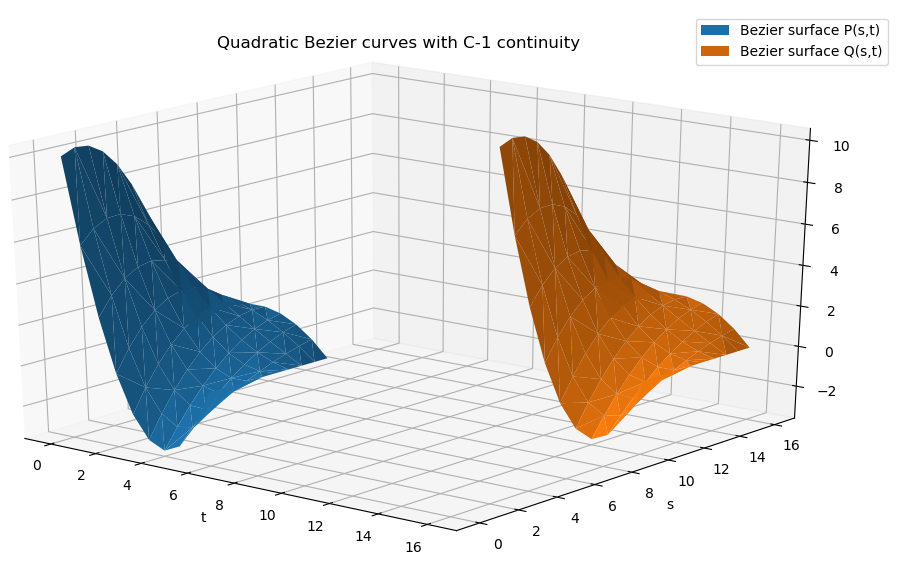
\includegraphics[scale=0.4]{resources/BezierSurfaceC-1.png} \label{fig:cs-1} 
  } \quad 
  \subfigure[Patches joined by \(C^{0}\) continuity]{% 
    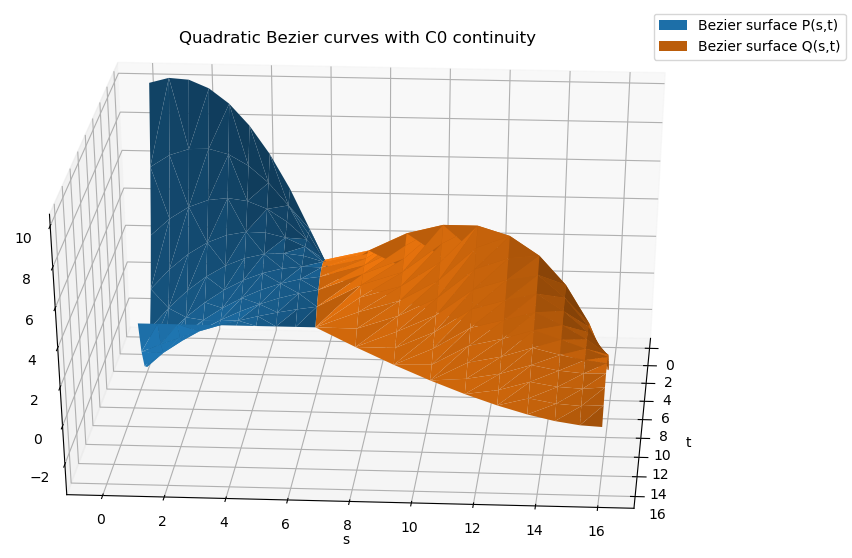
\includegraphics[scale=0.4]{resources/BezierSurfaceC0.png} \label{fig:cs0} 
  } \\
  \quad 
  \subfigure[Patches joined by \(C^{1}\) continuity]{% 
    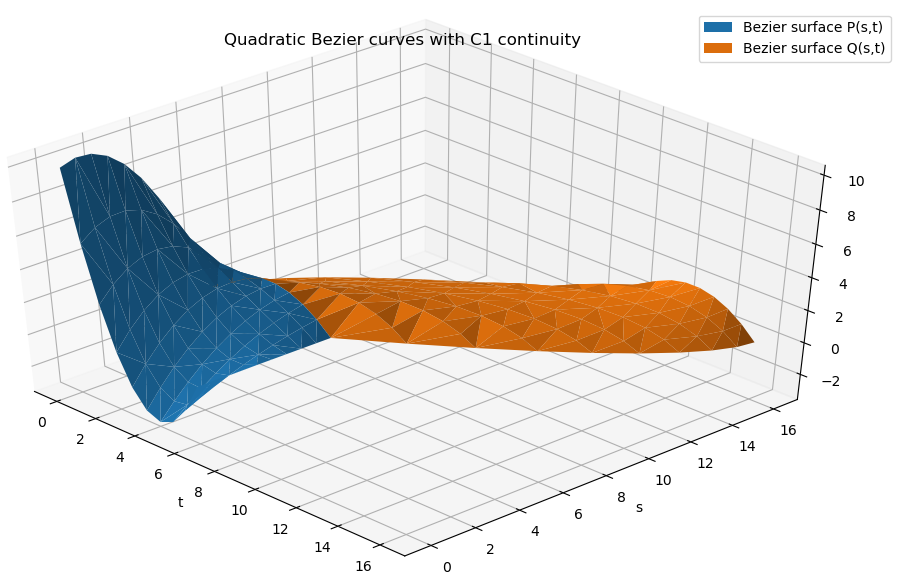
\includegraphics[scale=0.4]{resources/BezierSurfaceC1.png}
     \label{fig:cs1} 
  }
  \caption{Quadratic Bezier Patches \(P(s,t)\) and \(Q(s,t)\) joined by different continuities.} 
  \label{fig:bezierSurfacesJoined}
\end{figure}
\clearpage
\end{enumerate}

\item \textbf{(10 points)} This question asks you to generate a curve defined by the control points using the quadratic B\'{e}zier basis functions. You are given a circle.txt file. It has 16 vertices and 8 faces (line elements). Describe succinctly what you have done

Each face (element) of the mesh comprises of three vertices. For example circle.txt file shows that the second face comprises of vertices \{2, 3, 4\}. Using the parametrisation show in figure .
\textbf{Solution}

The first line of the text file represents the number of vertices and faces. Based on that we load up the vertices as \texttt{Point} objects into a dictionary and then faces into a dictionary, as \texttt{Face} objects which contain those \texttt{Point} objects. The curve to be generated is to be defined using the quadratic basis therefore the Face class contains those basis functions as $b0$, $b1$, and $b2$. 
\\ \\
Each face contains 3 points, these three points are used to draw a quadratic bezier curve using the quadratic bezier basis function. \\ \\
After loading up all faces, for each face we calculate its underlying curve \(F_i(t)\) where \(i\) represents the curve corresponding to face \(F_i\). \(\boldsymbol{F_i}_j\) represents the $j^{th}$ vertex of face \(F_i\). The parametric coordinate $t$ is interpolated to produce a smooth curve. The interpolation is done by increasing $t$ from 0 to 1 in steps of $0.0001$. We calculate the Bezier curve for each face by, 
\begin{equation}
\label{eq:face}
    F_i(t) = (1-t)^2 \boldsymbol{F_i}_0 + 2(1-t)(t)\boldsymbol{F_i}_1 + t^2\boldsymbol{F_i}_2 %\cite{NADNotes14} 
\end{equation}
The entire curve as shown in figure \ref{fig:BeziercurveQ2} is generated by combining the individual curves for all faces. 
\begin{figure}[ht]
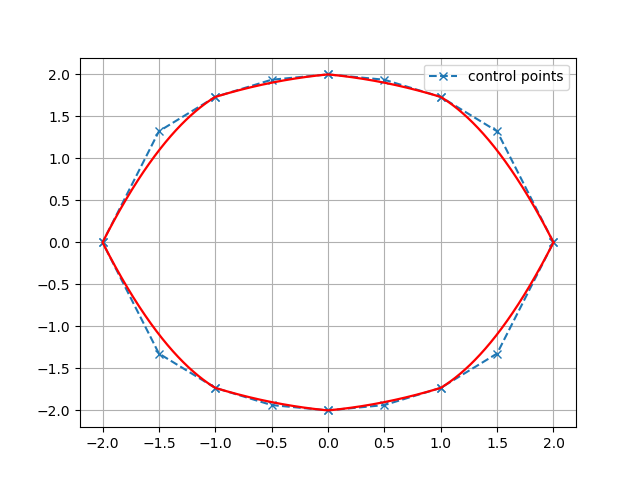
\includegraphics[scale=0.8]{resources/Q2_QBezBasis.png}  
\centering
\caption{Figure Generated using the control points and quadratic Bezier basis functions}
\label{fig:BeziercurveQ2}
\end{figure}
\item \textbf{(20 points)} You are now asked to generalise your algorithm in question 2 from curves to surfaces. Given the mesh for the one-eighth of a sphere in sphere.txt. The screenshot of the mesh is shown in Figure \ref{fig:sphereFig}
\begin{figure}
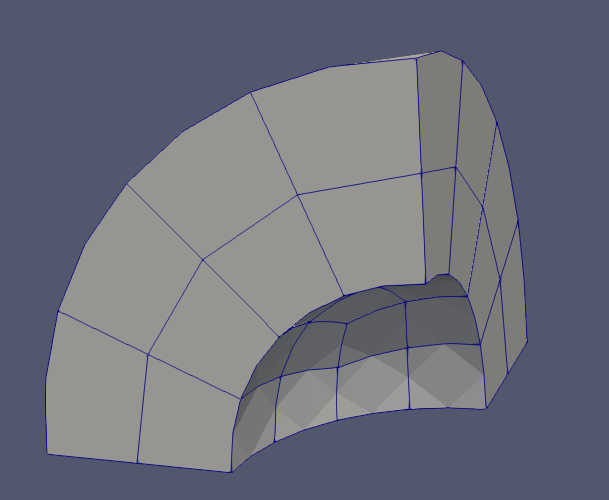
\includegraphics[scale=0.35]{resources/sphere.png} 
\centering
\caption{Mesh for the one-eighth of a sphere}
\label{fig:sphereFig}
\end{figure}
The 'sphere.txt' file has 224 vertices and 60 quadrilateral faces/elements. Each quadrilateral face/element comprises of 9 points. The quadrilateral in the sphere.txt numbers the vertices. Generate the surface represented by the mesh  using the quadratic B\'{e}zier basis functions.
\subsection*{Solution}
Each face contains 9 points, these nine points are used to draw a quadratic bezier patch using the quadratic bezier basis function for surfaces. \\ \\
After loading up all faces, for each face we calculate its underlying curve \(F_i(s,t)\) where \(i\) represents the patch corresponding to face \(F_i\). We calculate the Bezier patch for each face by, 
\begin{multline}
    \label{eq:sphere}
        F_i(s,t) = (1-s)^2[(1-t)^2 F_{0,0} + 2t(1-t) F_{0,1} + t^2 F_{0,2}] + \\ 2s(1-s)[(1-t)^2 F_{1,0} + 2t(1-t) F_{1,1} + t^2 F_{1,2}] + \\
        s^2[(1-t)^2 F_{2,0} + 2t(1-t) F_{2,1} + t^2 F_{2,2}]
\end{multline}
The entire patch as shown in figure \ref{fig:BezierSurfaceQ3} is generated by combining the individual patches for all faces. 
\begin{figure}[ht]
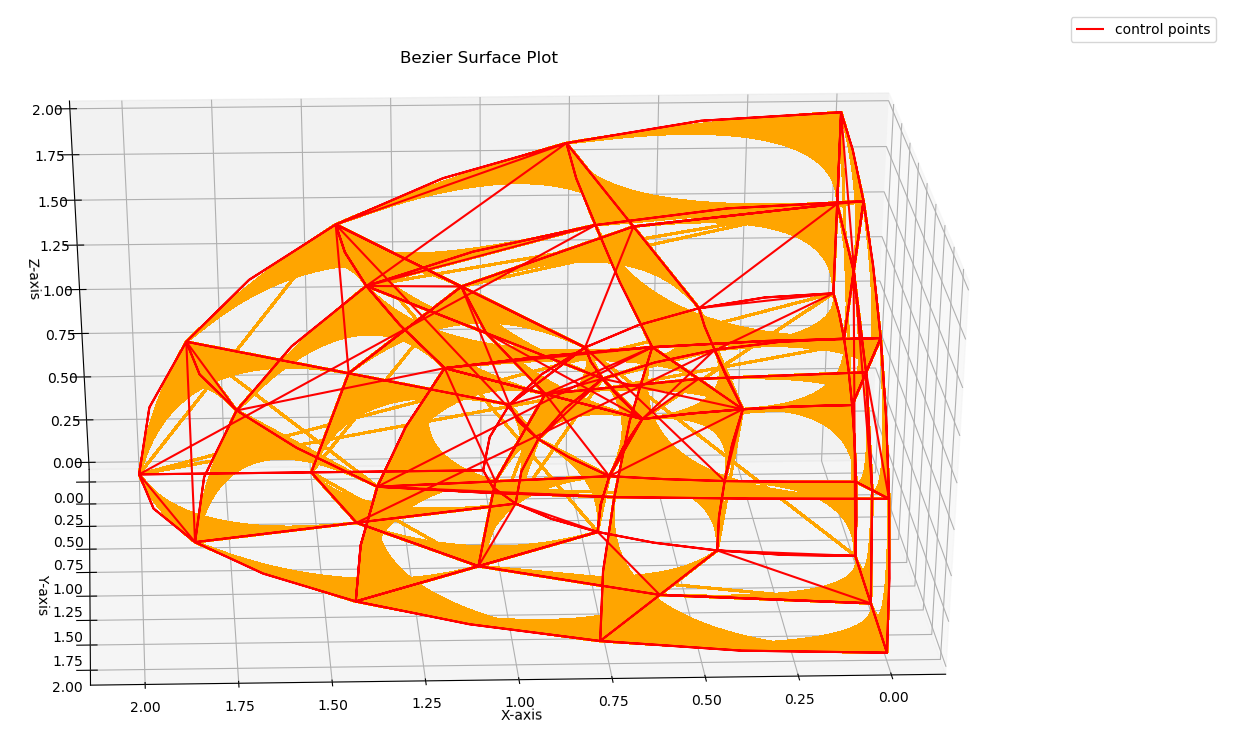
\includegraphics[scale=0.5]{resources/Q3_QBezSurface.png}  
\centering
\caption{$\frac{1}{8}$ Sphere generated using quadratic bezier patches}
\label{fig:BezierSurfaceQ3}
\end{figure}
\newpage
\begin{thebibliography}{}
    \bibitem{bezier} “Bezier curves.” [Online]. \\Available: https://www.cl.cam.ac.uk/teaching/2000/AGraphHCI/SMEG/node3.html. [Accessed: 25-Oct-2019].
\end{thebibliography}


\end{enumerate}
\end{document}